\documentclass[11pt]{article}
\usepackage{amsmath, amssymb, amscd, amsthm, amsfonts}
\usepackage{graphicx}
\usepackage{hyperref}
\usepackage{gensymb}

\oddsidemargin 0pt
\evensidemargin 0pt
\marginparwidth 40pt
\marginparsep 10pt
\topmargin -70pt
\headsep 10pt
\textheight 8.7in
\textwidth 6.65in
\linespread{1.2}

\title{Data Analytics Assignment-1: Mars Orbit}
\author{Anshul Shivhare}
\date{August 26, 2021}

\newtheorem{theorem}{Theorem}
\newtheorem{lemma}[theorem]{Lemma}
\newtheorem{conjecture}[theorem]{Conjecture}

\newcommand{\rr}{\mathbb{R}}

\newcommand{\al}{\alpha}
\DeclareMathOperator{\conv}{conv}
\DeclareMathOperator{\aff}{aff}

\begin{document}

\maketitle

\section{Formulation of the problem}\label{section-formulation}

\subsection{Model assumptions}
\begin{itemize}
    \item The Sun is the centre of our coordinate system (Sun is at the location (0, 0) in the ecliptic plane).
    \item Mars follows a circular orbit, with centre angle $c$ and distance $1$ from the Sun. That is, the centre of the orbit is at $(\cos{c}, \sin{c})$ in cartesian coordinates.
    \item The radius of the Mars orbit is $r$.
    \item The equant is located at $(e_1, e_2)$ in polar coordinates, or $(e_1 \cos{e_2}, e_1 \sin{e_2})$ in cartesian system.
    \item The reference longitude is given by angle $z$ with respect to the Aries.
    \item The angular velocity of Mars around the equant is $s$ degrees per day.
\end{itemize}

\subsection{Derivation of the angular error}

The model of Mars orbit can be visualised as in Figure 1 (only the first opposition is drawn for simplicity).  Here, $P_1$ refers to the position of Mars with respect to the equant, and $P_2$ is the opposition observation. The line from $P_2$ to Sun (Line 2) makes an angle $l$ with Aries, where $l$ is the heliocentric longitude of the first opposition. And, $P_1$ makes an angle $l + \delta$ with Aries (Line 1), so basically we want to find this angular error $\delta$.
\\
\\
Since the centre of the Mars orbit is $(\cos{c}, \sin{c})$, the equation of the circular orbit can be written as follows:
\begin{align*}
 &(x - \cos{c})^2 + (y - \sin{c})^2 = r^2\\
\Rightarrow & x^2 + y^2 - 2x\cos{c} -2y\sin{c} + 1 - r^2= 0
\end{align*}

\begin{figure}[h]
\centering
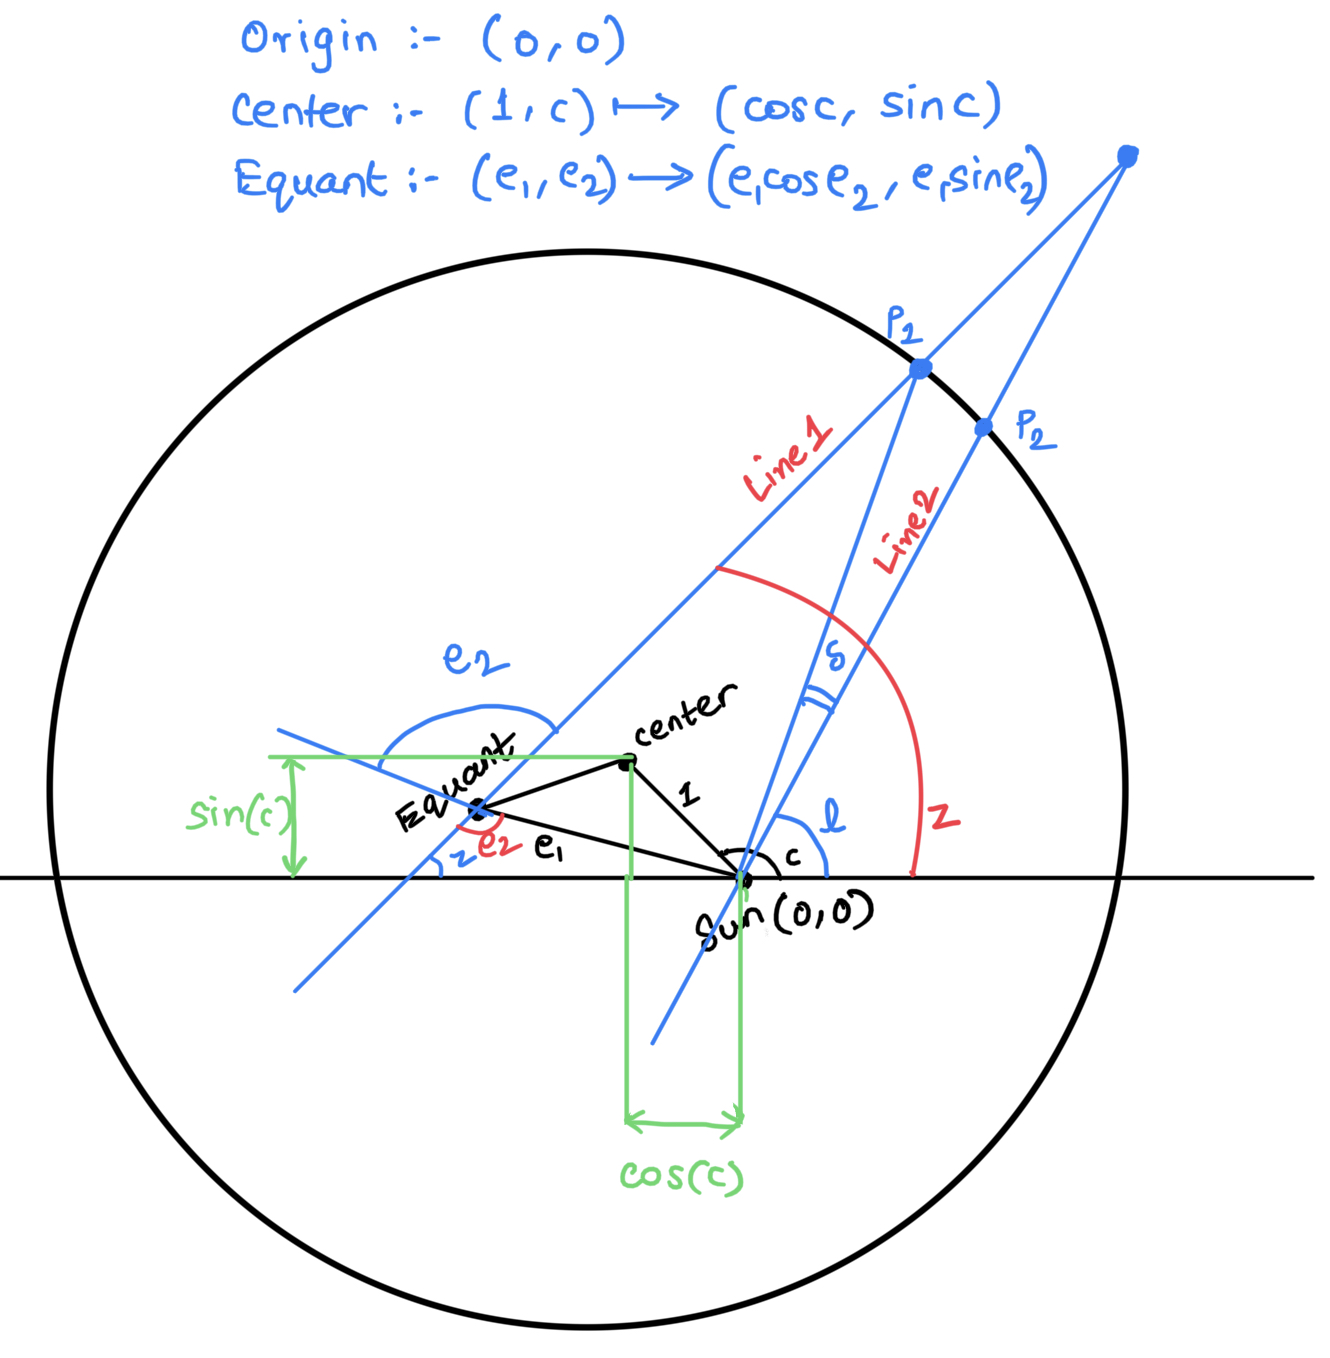
\includegraphics[width=0.66\textwidth]{file}
\caption{Example of a parametric plot ($\sin (x), \cos(x), x$)}
\end{figure}

The equation of Line 1 in Figure 1 can be written as follows:
\begin{align*}
 & y = m_1 x + c_1 \\
\Rightarrow & y = x \tan{z} + c_1 \text{     (Since the line makes angle $z$ with Aries)} \\
\Rightarrow & e_1 \sin{e_2} = e_1 \cos{e_2} \tan{z} + c_1 \text{    (Since equant also lies on the same line)} \\
\Rightarrow & c_1 = e_1 \sin{e_2} - e_1 \cos{e_2} \tan{z}
\end{align*}

Now we want to find the point of intersection of Line 1 with the orbit ($P_1$) in order to compute $\delta$. Substituting $y = x \tan{z} + c_1$ in the equation of the circular orbit, we get:
\begin{align*}
    & x^2 + (x \tan{z} + c_1)^2 - 2x\cos{c} - 2(x \tan{z} + c_1) \sin{c} + 1 - r^2 = 0 \\ 
    \Rightarrow & x^2 (1 + \tan^2{z}) + x (2 c_1 \tan{z} - 2 \cos{c} - 2\tan{z}\sin{c}) + (c_1^2 - 2 c_1 \sin{c} + 1 - r^2) = 0
\end{align*}

This is a quadratic equation of the form $ax^2 + bx + c = 0$, where
\begin{align*}
    & a = 1 + \tan^2{z} \\
    & b = 2 c_1 \tan{z} - 2 \cos{c} - 2\tan{z}\sin{c} \\
    & c = c_1^2 - 2 c_1 \sin{c} + 1 - r^2
\end{align*}

We solve this quadratic equation in order to get the $x$ and $y$ coordinates of the point $P_1$. Now, since the Sun is at the origin $(0, 0)$, the angle $(l + \delta)$ is nothing but $\tan^{-1}{\frac{y}{x}}$. Hence we can get $\delta$ by subtracting $l$ from this angle.
\begin{equation*}
    \delta = \tan^{-1}{\frac{y}{x}} - l
\end{equation*}

Apart from the formulation described here, we also have to handle some additional corner cases while writing code. For e.g., the above quadratic equation can have two roots (as there can be two points of intersection between a line and a circle), which we denote by $(x_1, y_1)$ and $(x_2, y_2)$ in the code. So in the code, we compute two angular errors $\delta_1$ and $\delta_2$, and we choose the minimum of these two as our final $\delta$. More details on the code structure is explained in the next section.

\section{Structure of the code}\label{section-code}

After reading the data from CSV file using pandas, the code has been divided into functions for simplicity, each of which are briefly described below. 

\begin{itemize}
    \item \textbf{get\_time\_diff:} This function computes the time differences between consecutive oppositions from raw data. This is needed, because time difference between oppositions multiplied by angular velocity would help to compute the equant angles for Mars at all oppositions.
    
    \item \textbf{get\_longitudes:} This function computes the heliocentric longitudes of Mars at oppositions, using the various columns given in the csv file. These longitudes will be used to compute $\delta$ later.
    
    \item \textbf{get\_data:} This function takes the file path as string input, and internally uses the \emph{get\_time\_diff} and \emph{get\_longitudes} functions, and vertically stacks together the time-differences and longitudes in a single variable called \emph{data}, which is returned. This \emph{data} can now be passed on to other functions as parameters.
    
    \item \textbf{find\_delta:} Given the coordinates of point-of-intersection $P_1$ as $(x,y)$ and corresponding heliocentric longitude, this function computes the angular error $\delta$ (difference between $\tan^{-1}(\frac{y}{x})$ and $l$). While computing $\tan^{-1}(\frac{y}{x})$, I have also taken care of the cases of angles lying in each of the four quadrants.
    
    \item \textbf{MarsEquantModel:} This function takes the model orbit parameters $c$, $r$, $e_1$, $e_2$, $z$ and $s$, and computes angular error $\delta$ for each opposition, using the  derivation which is explained above. The function returns the errors of each opposition, as well as the max error of all these errors.
    
    \item \textbf{bestOrbitInnerParams:} This function will take the values of $r$ and $s$ as inputs, and searches for the best other parameters for these fixed values of $r$ and $s$ over a feasible search space, using the previous function \emph{MarsEquantModel}.
    
    \item \textbf{bestS:} This function takes a fixed value of $r$ as input and searches for the optimal value of $s$ using gridsearch, and inside the code, it uses our previously defined function \emph{bestOrbitInnerParams}. It returns the optimal $s$ and corresponding errors.
    
    \item \textbf{bestR:} This function takes a fixed value of $s$ as input and searches for the optimal value of $r$ using gridsearch, and inside the code, it uses our previously defined function \emph{bestOrbitInnerParams}. It returns the optimal $r$ and corresponding errors.
    
    \item \textbf{bestMarsOrbitParams:} This function takes only the oppositions data as input, and searches for suitable values of both $r$ and $s$ using gridsearch, and returns the approximate optimal parameters which result in lowest angular error $\delta$.
\end{itemize}

\section{Observations}\label{section-observations}

\begin{itemize}
    \item Based on Moodle discussions and my own understanding of the problem, I initially estimated the model parameters as: c = 150\textdegree, r = 9.0, $e_1$ = 1.4, $e_2$ = 150\textdegree, z = 54\textdegree and s = 360/687\textdegree per day. For these parameters, the maximum angular error $\delta$ I got using \emph{MarsEquantModel} function was 3.98\textdegree.
    
    \item By using the functions for next 4 subproblems, I estimated the optimal parameters for my Mars orbit model. My final estimated optimal parameters are: \textbf{$c$ = 139.0, $r$ = 8.732, $e_1$ = 1.60, $e_2$ = 148.70, $z$ = 56.47, $s$ = 360 / 687}. And the corresponding maximum error is \textbf{0.40878 degrees (24.527 minutes)}. The corresponding errors for each opposition from 1st to 12th opposition are: [0.244, 0.308, 0.408, 0.394, 0.380, 0.408, 0.408, 0.003, 0.062, 0.048, 0.063, 0.036] (in degrees).
    
    \item I also tried doing more exhaustive grid search with more precision in parameters, but the estimated execution time for such large search-spaces was more than 24 hours, and it was difficult to run the code for such long durations on my personal laptop (sometimes there would be interruptions in the code in the middle of execution), hence I narrowed down my search and slightly reduced the precision in order to be able to practically run the code. Using these settings, the least angular error that I have managed to get is 24.5 minutes. 
\end{itemize}

\section{Instructions to run the code}\label{section-instructions}

\begin{itemize}
    \item First run the \emph{get\_data} function with the name and path of the csv file as input, and store it in a variable \emph{data}.
    \item Pass on this \emph{data} as parameter along with other numerical parameters in order to test the subsequent Mars orbit functions.
\end{itemize}

\end{document}
